\chapter{Indicadores de TIC de governo eletrônico}
\label{indicadores_tic_egov}

A ONU tem \href{https://publicadministration.un.org/egovkb/en-us/Data/ICT-in-government}{indicadores de TIC de governo eletrônico} como algo complementar ao \hyperref[egdi]{EGDI}. Os indicadores são, conforme \cite{ONU_ICT_in_government_indicators}:

\begin{itemize}
	\item Existência de estratégia nacional de governo eletrônico ou equivalente;
	\item Existência de identidade digital para acessar ou outra forma de autenticação requirida para poder acessar serviços online;
	\item Existência de um portal de compras governamentais.
\end{itemize}

Os resultados globais dos indicadores estão presentes nas figuras \ref{fig:national_government_strategy}, \ref{fig:national_identity} e \ref{fig:procurement_portal}.

\begin{figure}[H]
	\centering
	\caption{Indicador: Existência de estratégia nacional de governo eletrônico ou equivalente}
	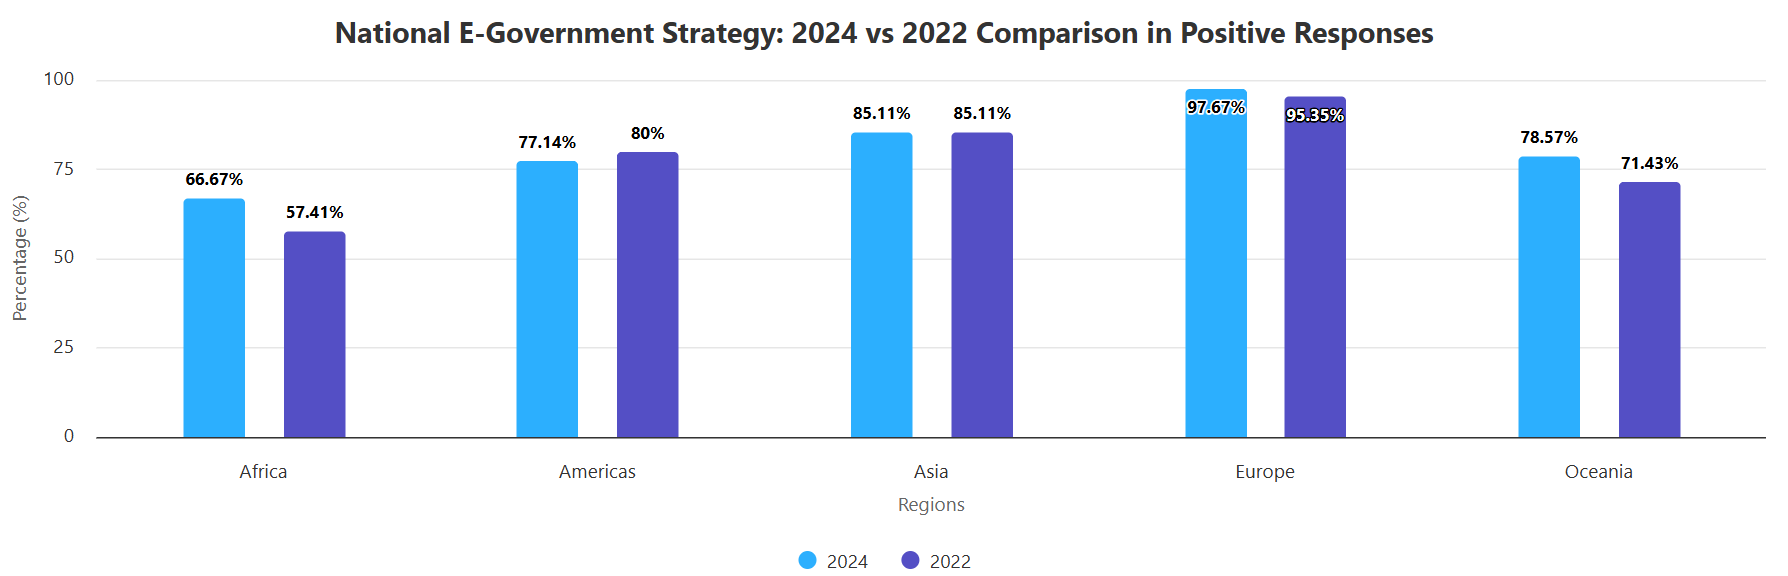
\includegraphics[width=1\linewidth]{figuras/ict_in_government/national_government_strategy}
	\label{fig:national_government_strategy}
	\footnotesize{Fonte: \cite{ONU_ICT_in_government_indicators}}
\end{figure}

\begin{figure}[H]
	\centering
	\caption{Indicador: Existência de identidade digital para acessar ou outra forma de autenticação requirida para poder acessar serviços online}
	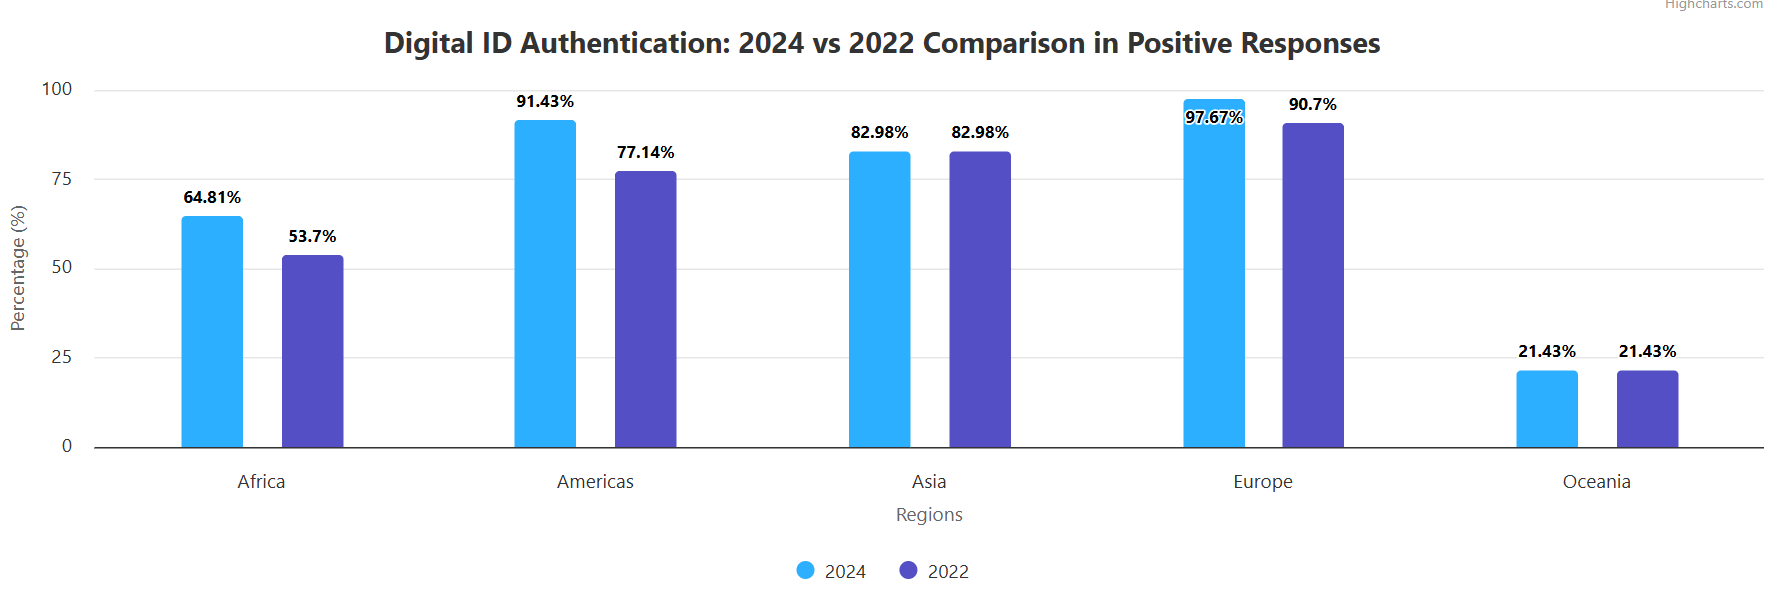
\includegraphics[width=1\linewidth]{figuras/ict_in_government/digital_identity}
	\label{fig:national_identity}
	\footnotesize{Fonte: \cite{ONU_ICT_in_government_indicators}}
\end{figure}

\begin{figure}[H]
	\centering
	\caption{Indicador: Existência de um portal de compras governamentais}
	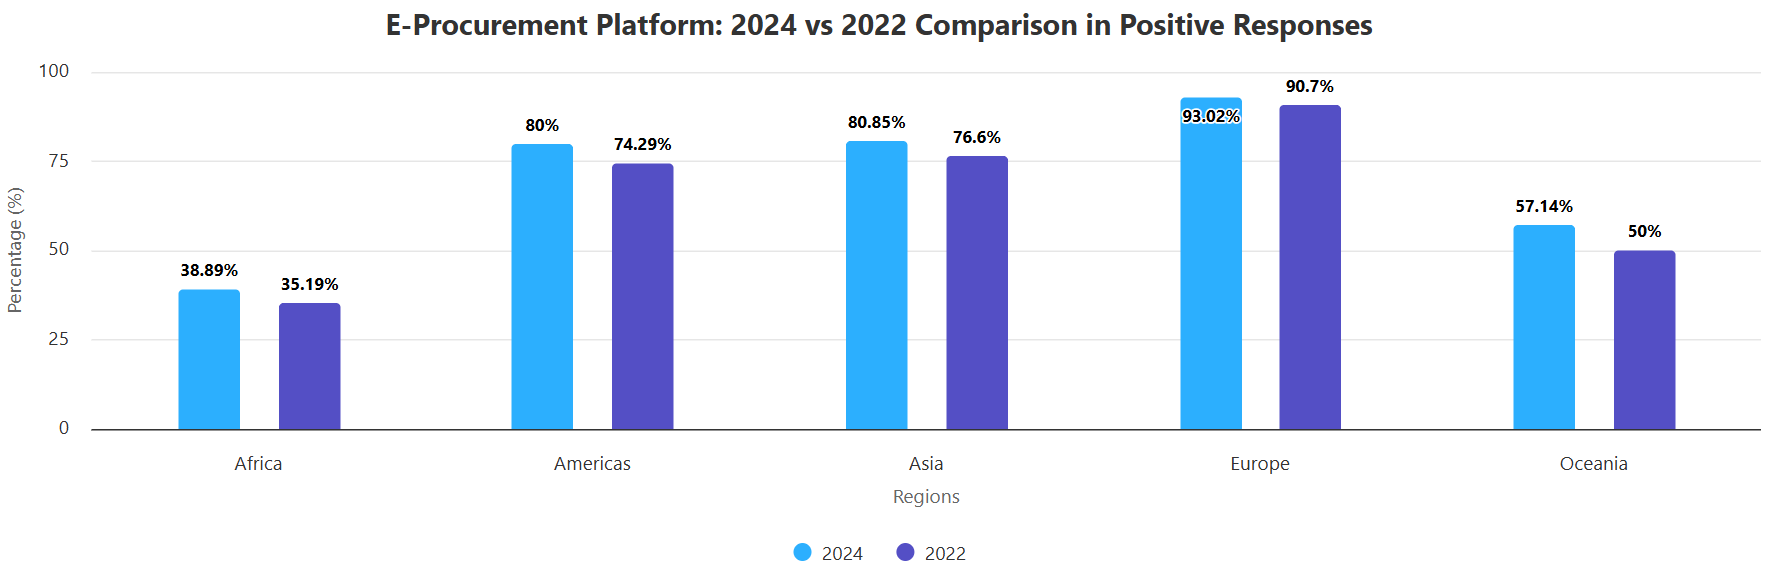
\includegraphics[width=1\linewidth]{figuras/ict_in_government/procurement_portal}
	\label{fig:procurement_portal}
	\footnotesize{Fonte: \cite{ONU_ICT_in_government_indicators}}
\end{figure}

Extraí-se das três figuras que a Europa foi o continente cujos mais respondem que têm seguem os indicadores, superando os 90\%. A Oceania foi o continente que menos implementou políticas de identidade digital para acesso a serviços online. África e Oceania tiveram um desempenho ruim na implementação de portais de compra governamentais. O continente americano apresentou bom desempenho nos três indicadores.

Como consequência da análise dos resultados presentes nas figuras \ref{fig:national_government_strategy}, \ref{fig:national_identity} e \ref{fig:procurement_portal}, buscou-se entender a seguinte situação registrada nos 2022 e 2024, anos em que os indicadores foram medidos: qual é a porcentagem de países que responderam nenhuma, uma, duas ou todas as perguntas. Elas usam sim ou não para confirmar a aplicação dos indicadores no país.

A resposta ao questionamento está presente na figura \ref{fig:indicators_answer}.

\begin{figure}[H]
	\centering
	\caption{Respostas positivas aos indicadores de TIC de governo eletrônico de 2024}
	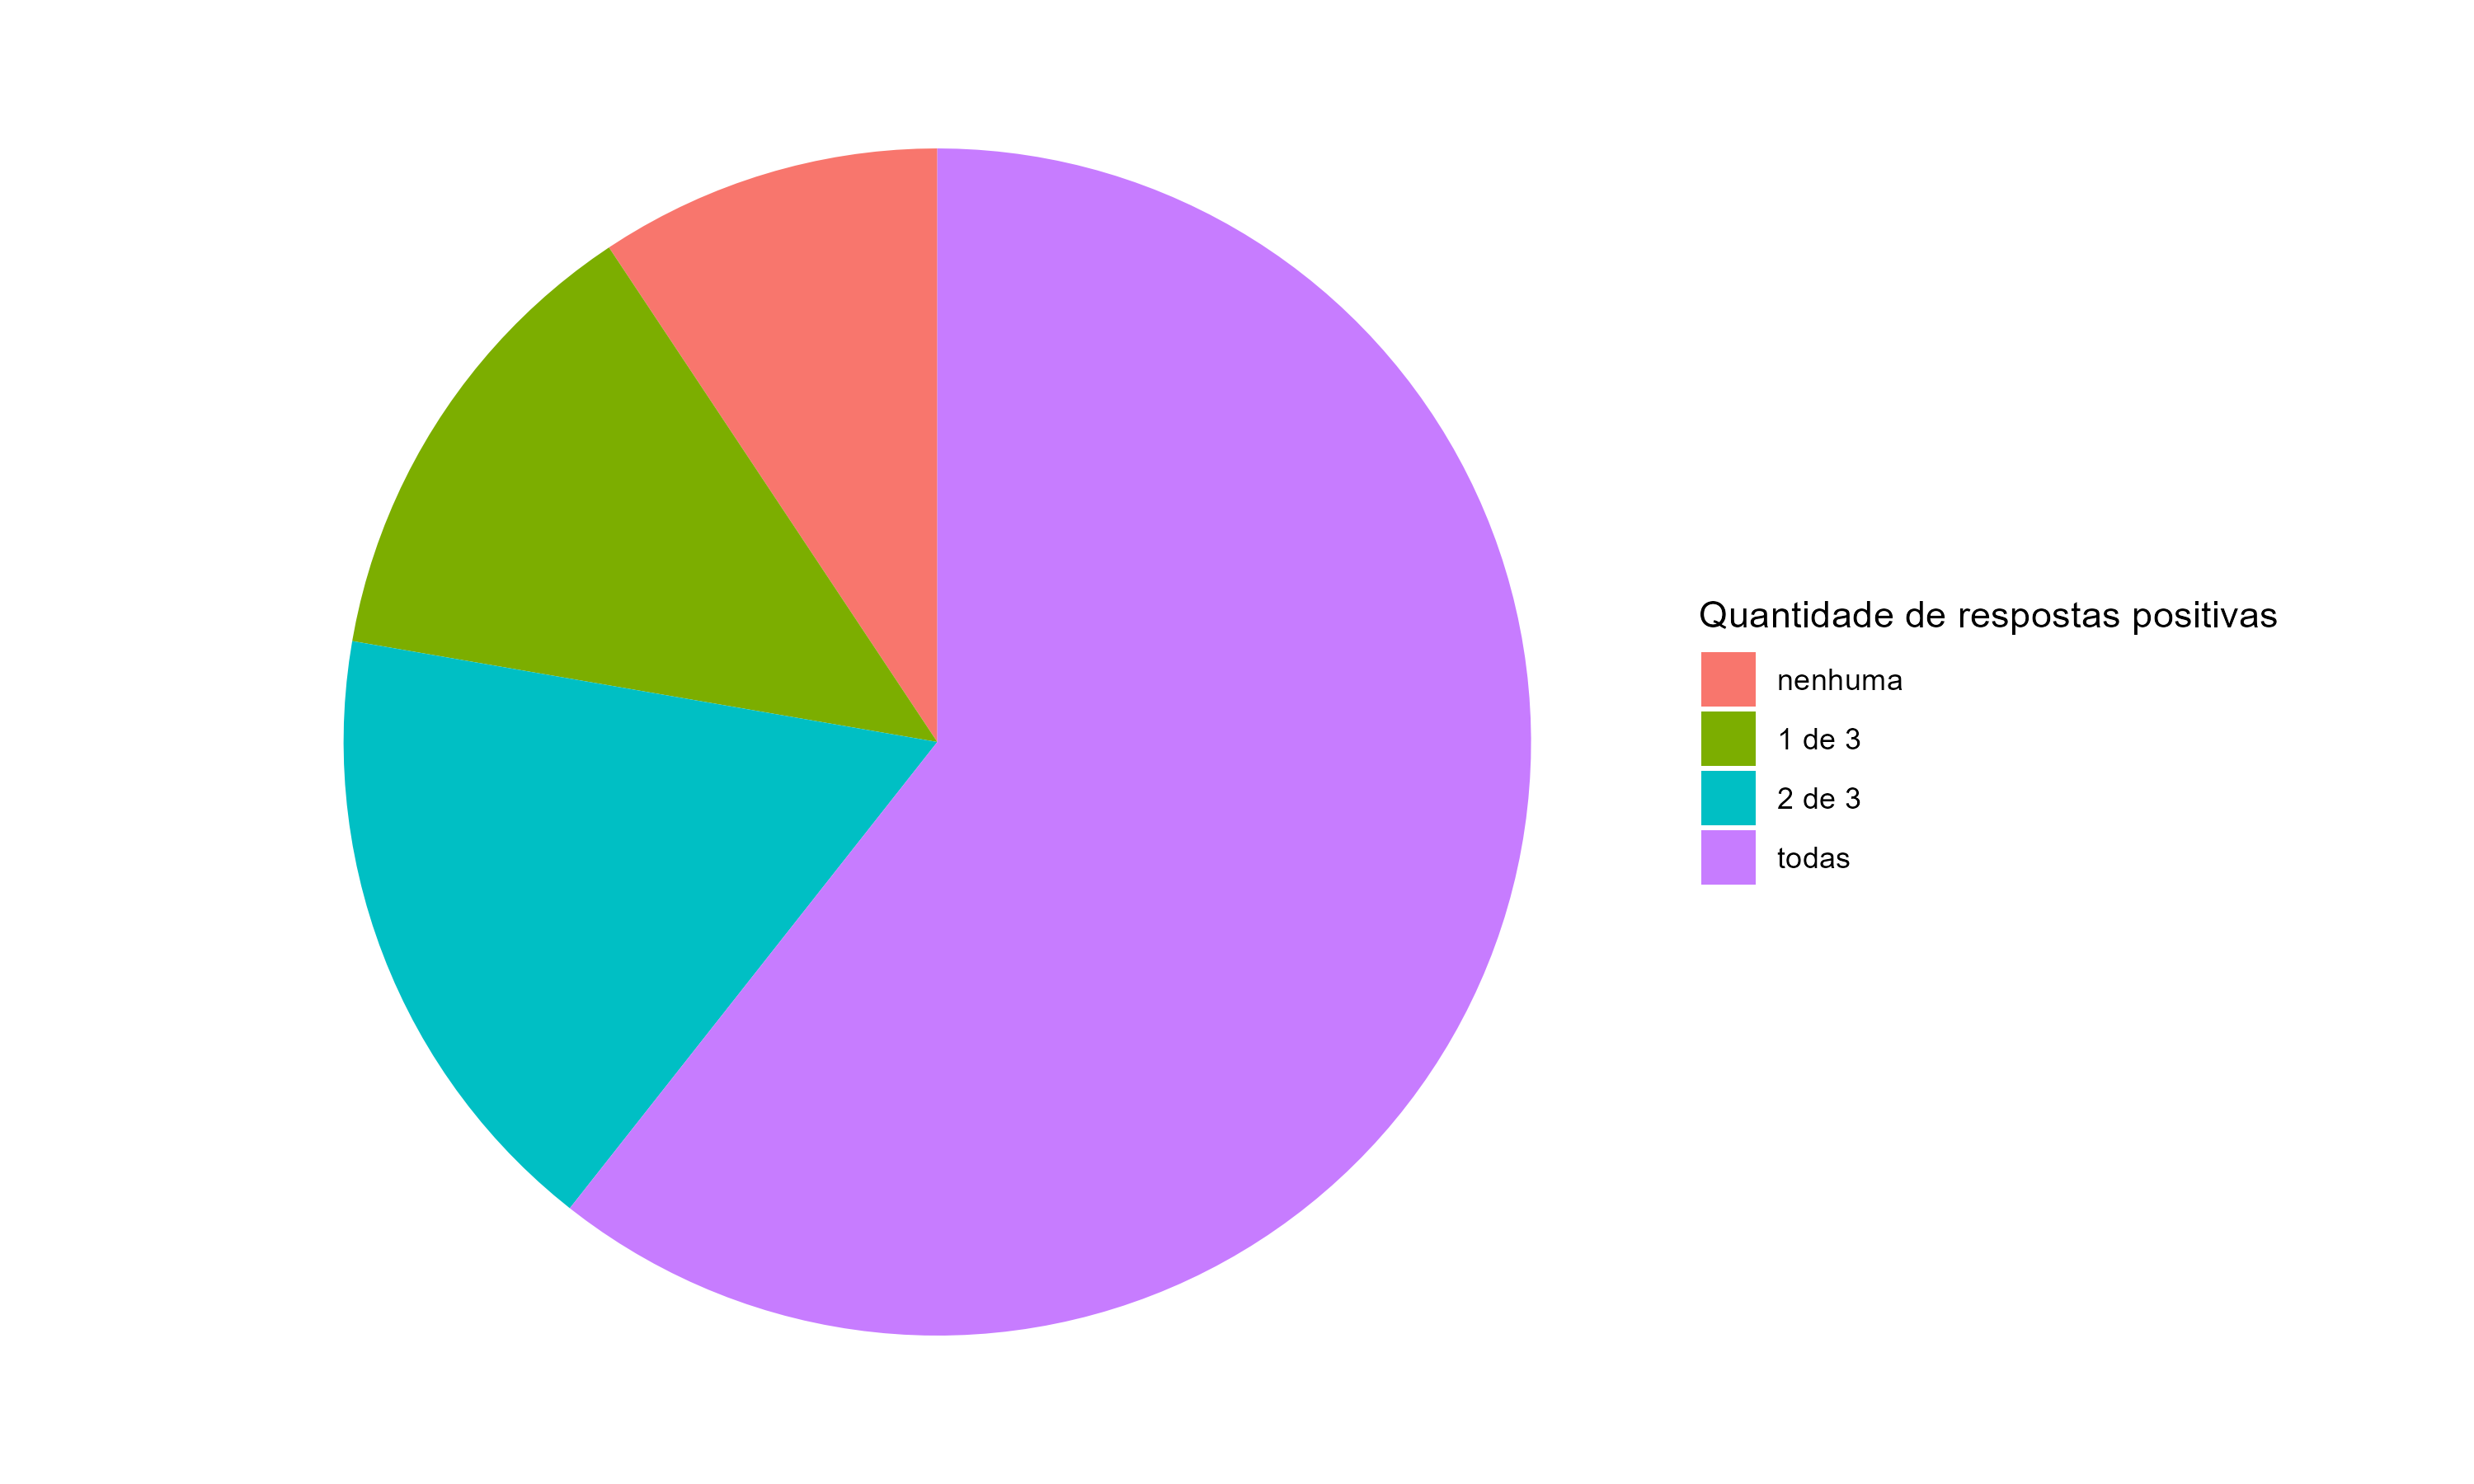
\includegraphics[width=1\linewidth]{figuras/ticegov_soma_respostas_positivas}
	\label{fig:ticegov_soma_respostas_positivas}
	\footnotesize{Fonte: \cite{ONU_ICT_in_government_indicators}}
\end{figure}

Em 2024, mais da metade dos países respondeu positivamente as três perguntas. O Brasil faz parte desse grupo, tal como a Rússia e China. Tal resultado índica que os mais da metado dos países estão investindo em TIC de governo eletrônico eletrônico em seus territórios.

\subsubsection{Coeficiente de correlação: indicadores de TIC de governo eletrônico  comparados com o PIB \textit{per capita} PPC e os gastos públicos (\% do PIB)}.

Com base na seção \ref{indicadores_tic_egov}, buscou-se entender se há correlação entre os indicadores de TIC de governo eletrônico e os PIB \textit{per capita} PPC e os gastos públicos (\% do PIB).

\begin{figure}[H]
	\centering
	\caption{Diagrama de Dispersão: indicadores de TIC de governo eletrônico e PIB \textit{per capita} PPC}
	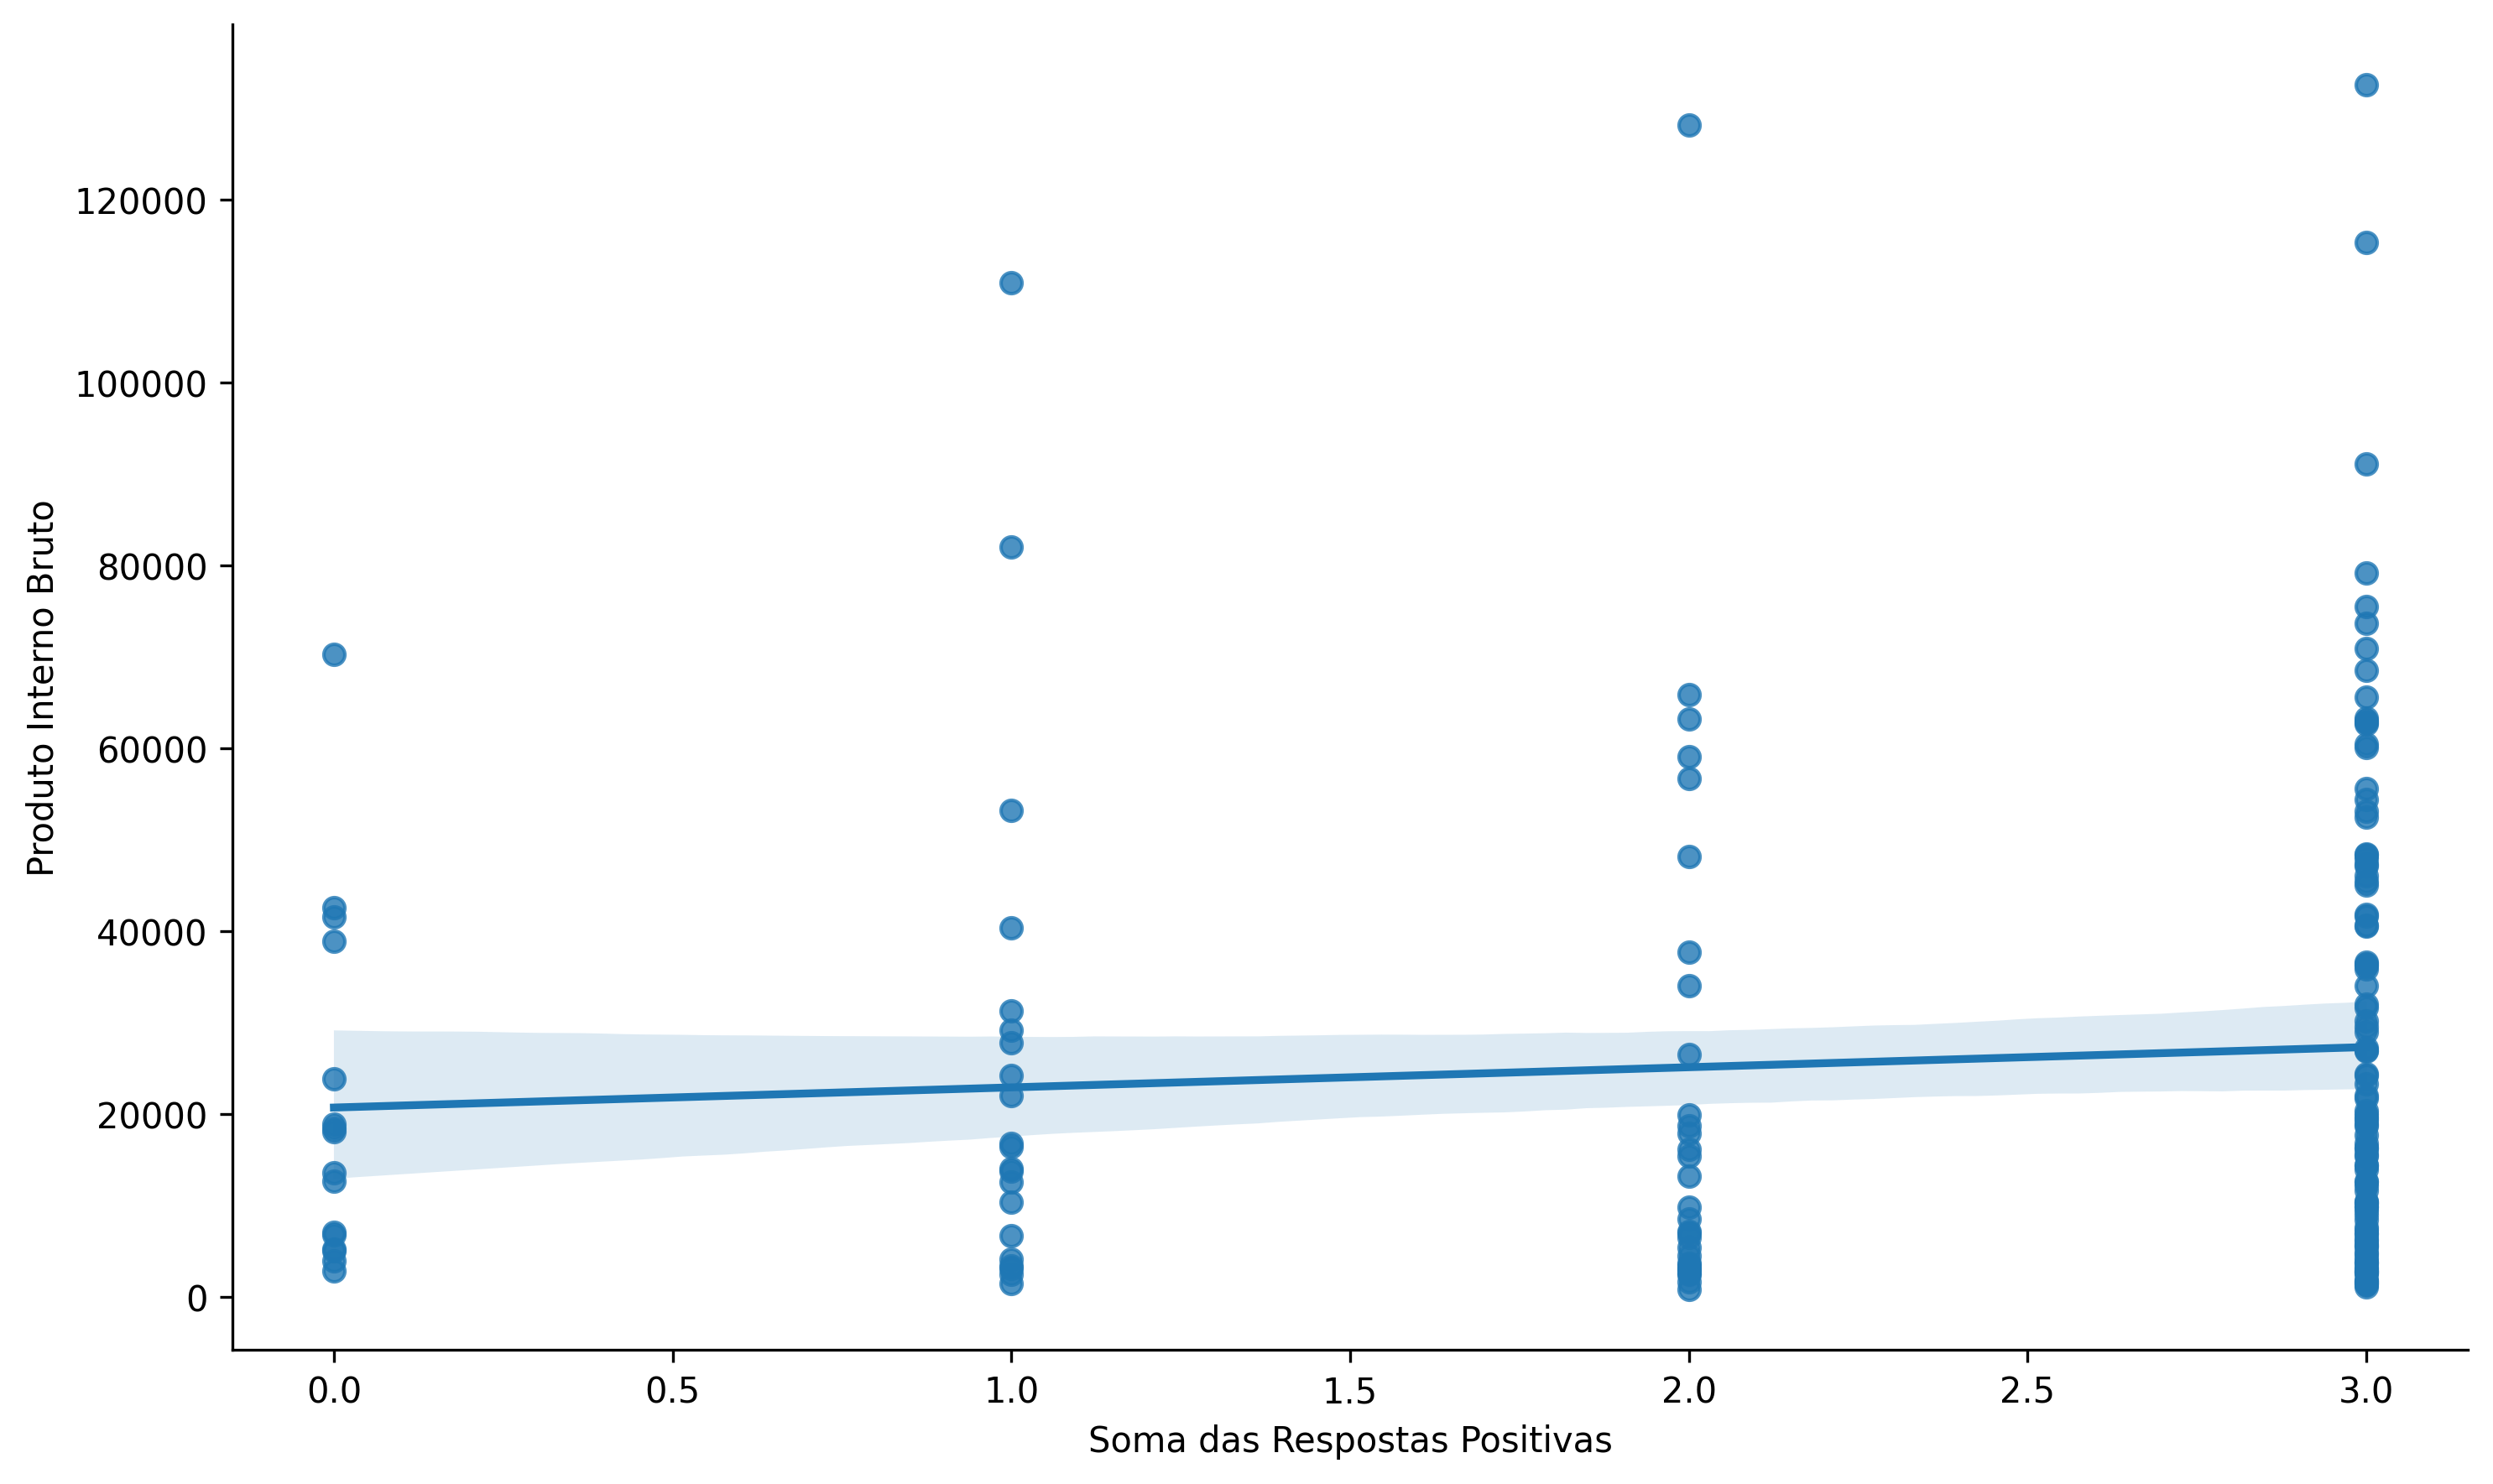
\includegraphics[width=1\linewidth]{figuras/ict_in_government/dispersao_ticegov_pib}
	\label{fig:dispersao_ticegov_pib}
	\footnotesize{Fonte: baseado em \cite{WB_pib_per_capita_países} e \cite{ONU_ICT_in_government_indicators}}
\end{figure}

Como o diagrama de dispersão presente na figura \ref{fig:dispersao_ticegov_pib} e apresenta grande dispersão em relação à tendência, optou-se pelo uso do coeficiente de correlação de Spearman. A alta dispersão em relação à tendência é um indicativo de um coeficiente de correlação neutro ou baixo. O coeficiente de correlação (0.1) indicam que os indicadores de TIC de governo eletrônico não são afetados pelo PIB \textit{per capita} PPC, e vice-versa.

Outra análise feita foi a comparação entre os indicadores de TIC de governo eletrônico e os gastos governamentais.

\begin{figure}[H]
	\centering
	\caption{Diagrama de Dispersão: indicadores de TIC de governo eletrônico e gastos públicos (\% do PIB)}
	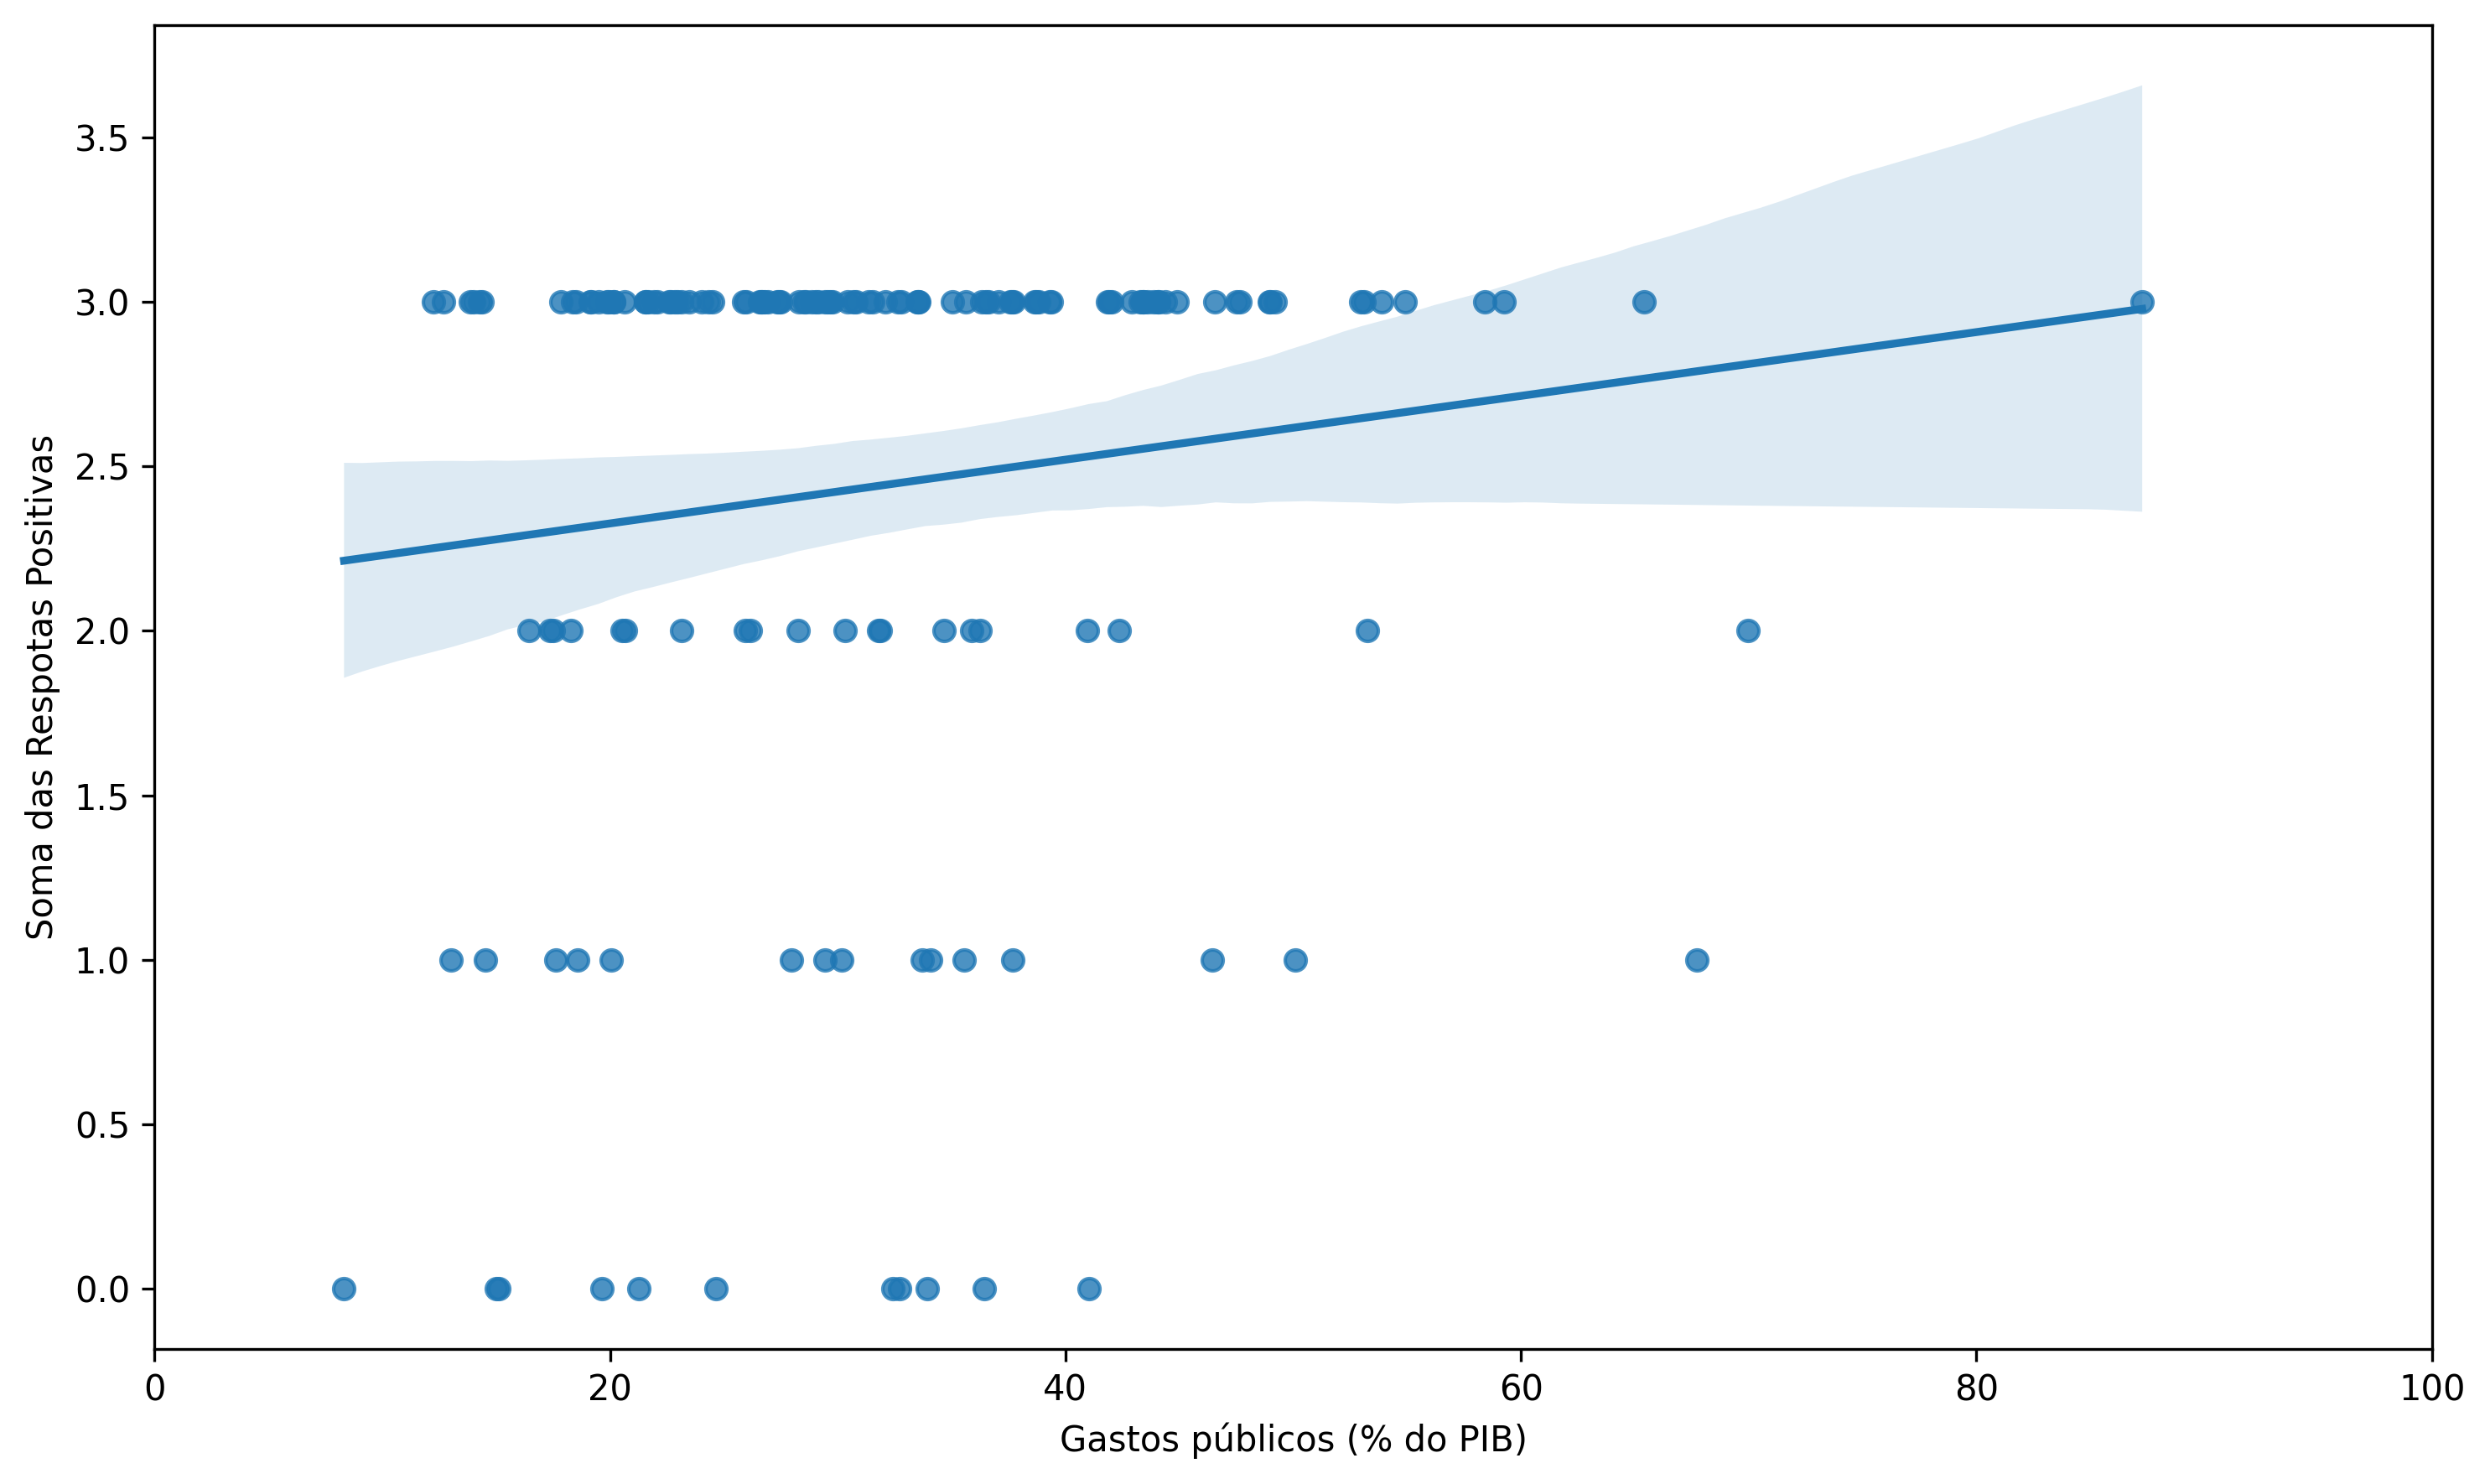
\includegraphics[width=1\linewidth]{figuras/ict_in_government/dispersao_ticegov_govexpenditure}
	\label{fig:dispersao_ticegov_govexpenditure}
	\footnotesize{Fonte: baseado em \cite{FMI_gov_expenditure} e \cite{ONU_ICT_in_government_indicators}}
\end{figure}

Para compreender melhor o diagrama de dispersão, foi usado o coeficiente de correlação de Spearman. A sua escolha foi motivada pela grande presença de pontos extremos. O coeficiente de correlação encontrada foi 0.23. O referido coeficiente indica uma correlação positiva muito fraca entre os gastos do governo e a soma das respostas positivas. 